\section{Modelo SM-CFHR}\label{sec:modelo}

El estimador \textbf{SM-CFHR} (\textit{Structured Monotone Capacity-Factor Huber Regressor}) opera íntegramente en el espacio adimensional del factor de capacidad y reconstruye las predicciones en unidades de energía física al finalizar la inferencia. La Figura~\ref{fig:sm_cfhr_arq} sintetiza el flujo completo desde el panel de entrenamiento hasta la proyección física.

\begin{figure}[!htbp]
\centering
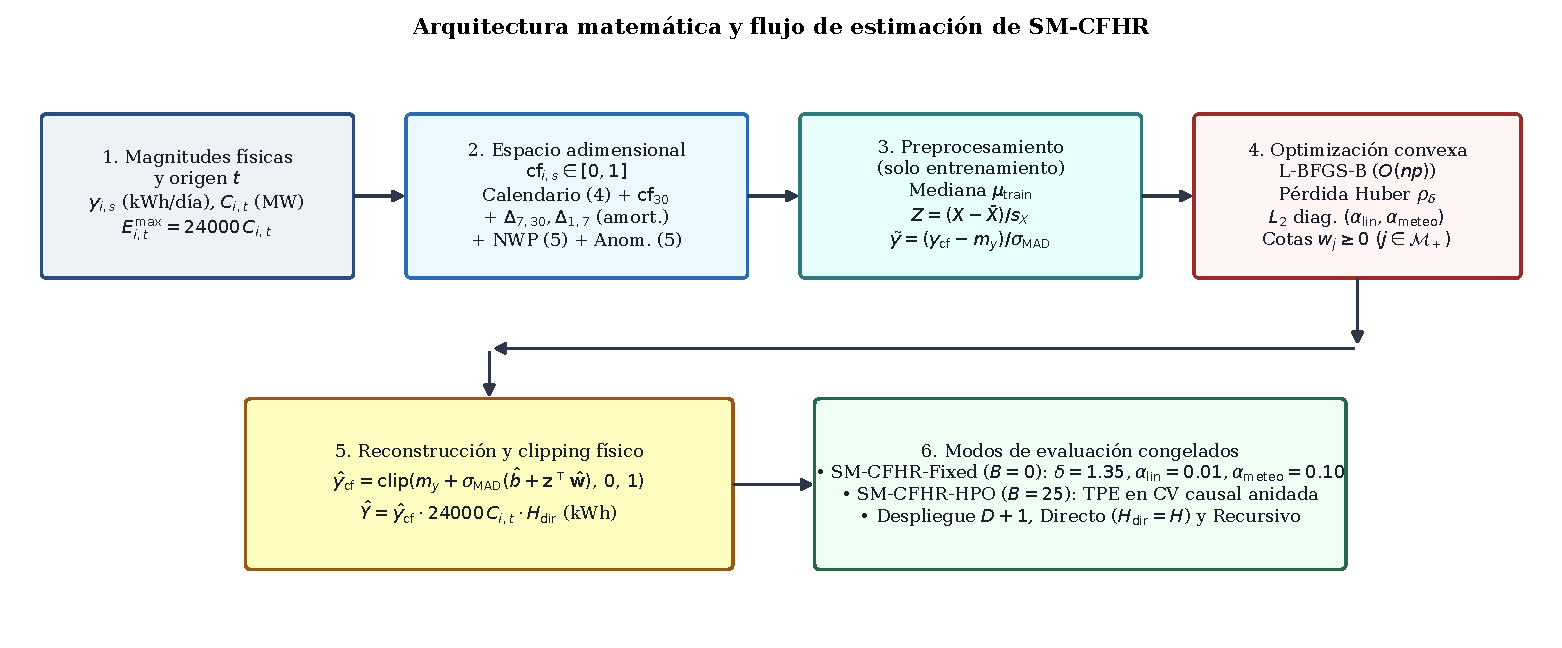
\includegraphics[width=0.98\textwidth]{figures/fig_sm_cfhr_arquitectura.pdf}
\caption{Arquitectura matemática de SM-CFHR: normalización causal por capacidad vigente, preprocesamiento sin fuga en entrenamiento, optimización convexa L-BFGS-B con pérdida de Huber y regularización $L_2$ diferenciada, y reconstrucción física acotada.}
\label{fig:sm_cfhr_arq}
\end{figure}

\subsection{Preprocesamiento en entrenamiento y escalado robusto MAD}

Sea $\mathcal{D}_{\mathrm{train}} = \{(\mathbf{x}_k, y_k)\}_{k=1}^n$ el conjunto de entrenamiento válido del pliegue (filtrando filas con $E^{\max}_k > 0$ y objetivo finito), con matriz de predictores $X \in \mathbb{R}^{n \times p}$ construida según la Sección~\ref{sec:conjuntos} ($p=7$ sin meteorología; $p=17$ con meteorología) y vector de factores de capacidad objetivo $\mathbf{y} \in [0,1]^n$ definido por \eqref{eq:cf_diario} o \eqref{eq:y_directo}. Todas las estadísticas de preprocesamiento se estiman exclusivamente sobre $\mathcal{D}_{\mathrm{train}}$:
\begin{enumerate}
    \item \textbf{Imputación por mediana:} cualquier valor no finito en la columna $j$ de $X$ se reemplaza por la mediana muestral $\mu_j = \mathrm{mediana}_k(X_{kj})$ calculada en $\mathcal{D}_{\mathrm{train}}$ (con respaldo $0$ si toda la columna es faltante), obteniendo $X^{\mathrm{imp}} \in \mathbb{R}^{n \times p}$.
    \item \textbf{Estandarización de predictores:} se calculan la media $\bar{x}_j = \frac{1}{n}\sum_{k=1}^n X^{\mathrm{imp}}_{kj}$ y la desviación estándar $s_j = \big(\frac{1}{n}\sum_{k=1}^n (X^{\mathrm{imp}}_{kj} - \bar{x}_j)^2\big)^{1/2}$. Para evitar inestabilidad numérica en columnas constantes, se define la escala efectiva $\tilde{s}_j = s_j$ si $s_j > 10^{-8}$ y $\tilde{s}_j = 1$ en caso contrario, produciendo la matriz estandarizada $Z \in \mathbb{R}^{n \times p}$ con entradas $Z_{kj} = (X^{\mathrm{imp}}_{kj} - \bar{x}_j)/\tilde{s}_j$.
    \item \textbf{Escalado robusto de la respuesta:} para que el umbral de transición $\delta > 0$ de la pérdida de Huber actúe en unidades adimensionales comparables entre centrales y estaciones, la respuesta se centra mediante la mediana $m_y = \mathrm{mediana}(\mathbf{y})$ y se escala mediante la desviación absoluta mediana $\mathrm{MAD}(\mathbf{y}) = \mathrm{mediana}(|\mathbf{y} - m_y|)$:
    \begin{equation}
    \sigma_y := \begin{cases}
    \max\{1{,}4826\,\mathrm{MAD}(\mathbf{y}),\; 10^{-6}\} & \text{si } \mathrm{MAD}(\mathbf{y}) > 0, \\
    \max\{\operatorname{std}(\mathbf{y}),\; 10^{-6}\} & \text{si } \mathrm{MAD}(\mathbf{y}) = 0,
    \end{cases}
    \qquad
    \tilde{y}_k := \frac{y_k - m_y}{\sigma_y}.
    \label{eq:mad_scale}
    \end{equation}
    La constante $1{,}4826 = 1/\Phi^{-1}(0{,}75)$ hace consistente a $\sigma_y$ con la desviación estándar bajo normalidad; el estimador MAD clásico posee punto de ruptura asintótico del $50\%$ \cite{rousseeuw1993mad}. En la implementación en NumPy (\texttt{\_robust\_target\_stats}), $m_y$ y $\mathrm{MAD}(\mathbf{y})$ se calculan mediante \texttt{np.median}, y cuando $\mathrm{MAD}(\mathbf{y}) = 0$ (cuando al menos la mitad de las observaciones coincide exactamente en $m_y$, contaminación por implosión) se activa el respaldo mediante la desviación estándar poblacional \texttt{np.std(..., ddof=0)} con piso numérico $10^{-6}$. Dado que la desviación estándar tiene punto de ruptura $0\%$ frente a valores atípicos, \emph{no} se demuestra ni se atribuye un punto de ruptura incondicional del $50\%$ al procedimiento compuesto por tramos \eqref{eq:mad_scale}.
\end{enumerate}

\subsection{Función objetivo, regularización estructurada y restricciones de signo}

Denotemos por $\mathbf{z}_k \in \mathbb{R}^p$ la $k$-ésima fila de $Z$. SM-CFHR estima un intercepto no penalizado $b \in \mathbb{R}$ y un vector de coeficientes $\mathbf{w} \in \mathbb{R}^p$ resolviendo el programa convexo:
\begin{equation}
\min_{b \in \mathbb{R},\; \mathbf{w} \in \mathcal{C}} \; J(b, \mathbf{w}) := \frac{1}{n}\sum_{k=1}^{n} \rho_\delta\!\left(\tilde{y}_k - b - \mathbf{z}_k^\top \mathbf{w}\right) + \frac{1}{2}\mathbf{w}^\top D_\alpha \mathbf{w},
\label{eq:objetivo_smcfhr}
\end{equation}
donde $\rho_\delta : \mathbb{R} \to \mathbb{R}_{\ge 0}$ es la pérdida de Huber con umbral $\delta > 0$,
\begin{equation}
\rho_\delta(r) := \begin{cases}
\frac{1}{2} r^2 & \text{si } |r| \le \delta, \\
\delta\left(|r| - \frac{1}{2}\delta\right) & \text{si } |r| > \delta,
\end{cases}
\label{eq:huber}
\end{equation}
la matriz diagonal $D_\alpha = \diag(d_1,\dots,d_p)$ asigna penalizaciones cuadráticas diferenciadas por familia de predictores,
\begin{equation}
d_j := \begin{cases}
\alpha_{\mathrm{meteo}} & \text{si } j \in \mathcal{G}_{\mathrm{meteo}}, \\
\alpha_{\mathrm{lin}} & \text{si } j \notin \mathcal{G}_{\mathrm{meteo}},
\end{cases}
\label{eq:d_alpha}
\end{equation}
siendo $\mathcal{G}_{\mathrm{meteo}} = \{8,\dots,17\}$ el bloque de variables meteorológicas y anomalías ($\mathcal{G}_{\mathrm{meteo}} = \emptyset$ cuando no hay meteorología), y el conjunto factible $\mathcal{C} \subseteq \mathbb{R}^p$ impone restricciones de no negatividad sobre el subconjunto de índices físicamente monótonos $\mathcal{M}_+$:
\begin{equation}
\mathcal{C} := \{\mathbf{w} \in \mathbb{R}^p : w_j \ge 0 \;\forall j \in \mathcal{M}_+\},
\quad
\mathcal{M}_+ = \begin{cases}
\{5, 8\} \text{ ($\mathrm{cf}_{30}$ e irradiación pronosticada)} & \text{con clima}, \\
\{5\} \text{ ($\mathrm{cf}_{30}$)} & \text{sin clima}.
\end{cases}
\label{eq:conjunto_factible}
\end{equation}

Desde el punto de vista estadístico, \eqref{eq:objetivo_smcfhr} extiende la regresión Ridge \cite{hoerl1970} y los híbridos robustos analizados por Owen~\cite{owen2007} en dos direcciones específicas del problema fotovoltaico. Por un lado, $D_\alpha$ permite aplicar una contracción moderada ($\alpha_{\mathrm{lin}}$) sobre la dinámica autorregresiva y el calendario, mientras regula con mayor intensidad ($\alpha_{\mathrm{meteo}}$) las variables NWP para mitigar el sobreajuste ante la degradación meteorológica de mediano plazo. Por otro lado, las cotas $w_j \ge 0$ para $j \in \mathcal{M}_+$ impiden que la colinealidad entre predictores produzca pendientes negativas físicamente espurias respecto al nivel base reciente o a la irradiación pronosticada.

El modelo se evalúa bajo dos presupuestos experimentales bien delimitados:
\begin{itemize}
    \item \textbf{SM-CFHR-Fixed ($B=0$):} configuración congelada con $\delta = 1{,}35$, $\alpha_{\mathrm{lin}} = 0{,}01$ y $\alpha_{\mathrm{meteo}} = 0{,}10$ (en ausencia de meteorología, $d_j = \alpha_{\mathrm{lin}}$ para todo $j$), sin búsqueda interna de hiperparámetros.
    \item \textbf{SM-CFHR-HPO ($B=25$):} optimización bayesiana TPE mediante Optuna dentro de cada pliegue externo sobre el espacio continuo $\delta \in [0{,}5, 3{,}0]$, $\alpha_{\mathrm{lin}} \in [10^{-4}, 1{,}0]$ (escala logarítmica) y, cuando hay meteorología, $\alpha_{\mathrm{meteo}} \in [10^{-3}, 10{,}0]$ (escala logarítmica). En los escenarios recursivos, la validación interna evalúa cada candidato mediante el mismo Algoritmo~\ref{alg:rollout} de despliegue causal exacto.
\end{itemize}

\subsection{Reconstrucción física y modos de despliegue}

Para un vector de consulta $\mathbf{x}_q \in \mathbb{R}^p$, se aplica la imputación $\mu_j$ y la estandarización $\mathbf{z}_q = (\mathbf{x}^{\mathrm{imp}}_q - \bar{\mathbf{x}})/\tilde{\mathbf{s}}$ con los parámetros del entrenamiento. A partir de la solución óptima $(\hat{b}, \hat{\mathbf{w}})$, el factor de capacidad y la energía física predichos se obtienen mediante:
\begin{equation}
\widehat{\mathrm{cf}}_q := \clip\!\left(m_y + \sigma_y \big(\hat{b} + \mathbf{z}_q^\top \hat{\mathbf{w}}\big),\; 0,\; 1\right),
\qquad
\hat{y}_q := \widehat{\mathrm{cf}}_q \cdot 24\,000\,C_{i,t} \cdot H_{\mathrm{dir}} \quad (\text{kWh}),
\label{eq:pred_fisica}
\end{equation}
con respaldo al promedio histórico $\bar{y}^{(30)}_{i,t}\,H_{\mathrm{dir}}$ si $C_{i,t}$ no fuese finita, acotado al intervalo físico $[0, 24\,000\,H_{\mathrm{dir}}\,C_{i,t}]$.

La Figura~\ref{fig:despliegue_mh} contrasta los tres modos de despliegue: (1) $D+1$ ($H=1$, $H_{\mathrm{dir}}=1$), que evalúa \eqref{eq:pred_fisica} una sola vez; (2) el esquema directo acumulado ($H \in \{7,14,21,28\}$, $H_{\mathrm{dir}}=H$), que entrena y predice directamente sobre la energía total de la ventana $[t+1, t+H]$ sin realimentación; y (3) el esquema recursivo multihorizonte ($H \in \{7,14,21,28\}$, $H_{\mathrm{dir}}=1$), que entrena en $h=1$ e itera el Algoritmo~\ref{alg:rollout} realimentando exclusivamente sus propias predicciones. Conviene subrayar que, aunque el ajuste interno \eqref{eq:objetivo_smcfhr} es un programa convexo, la composición recursiva de $H$ pasos realimentando $\hat{y}_{i,t_0+h \mid t_0}$ es una función no lineal y no convexa de los parámetros.

\begin{figure}[!htbp]
\centering
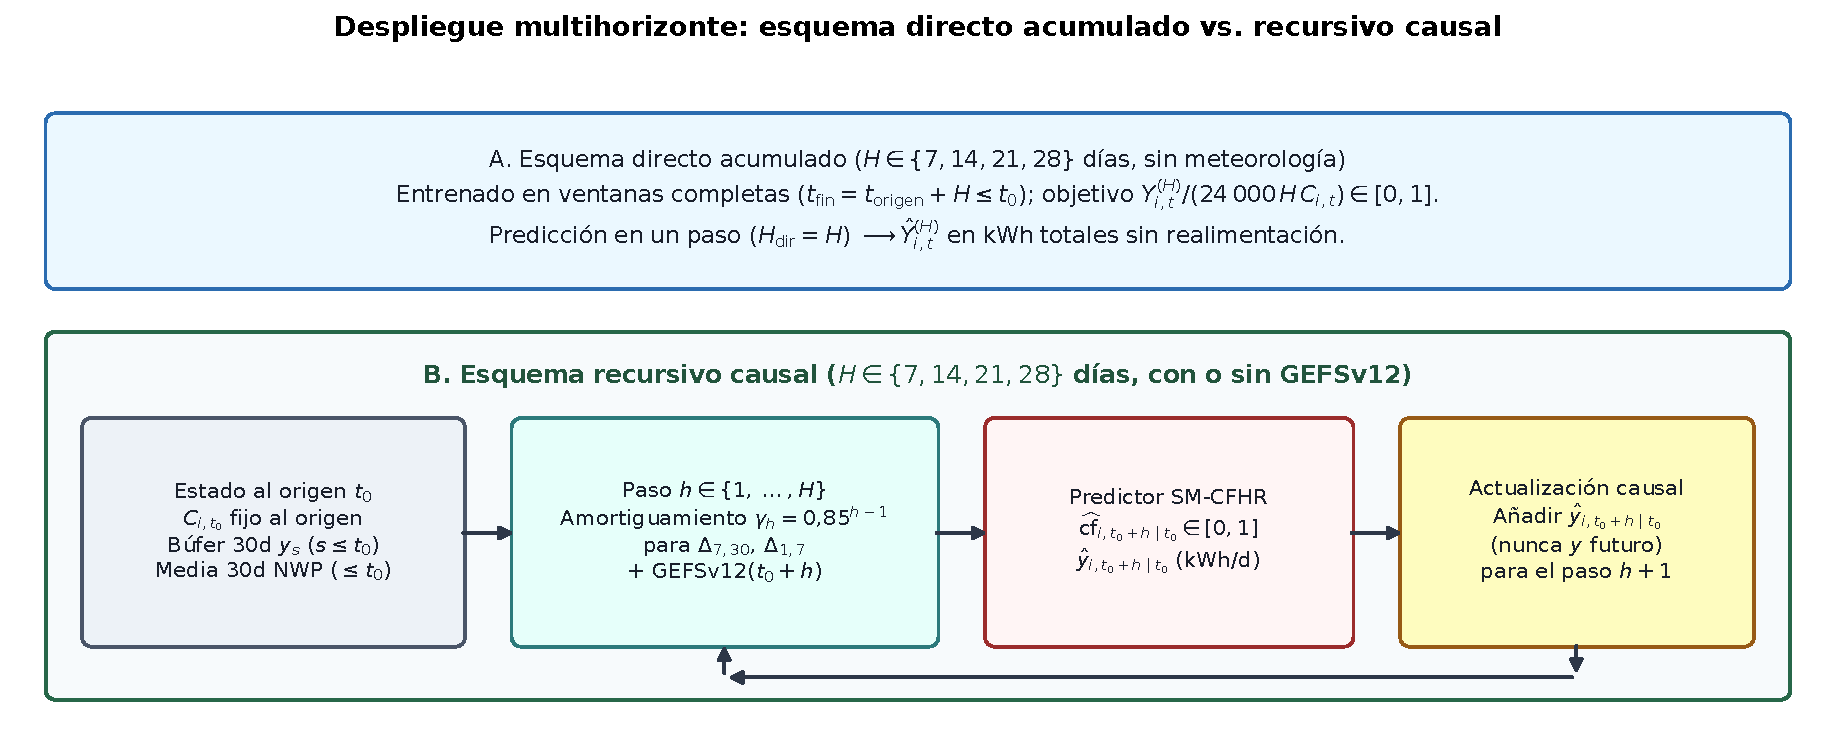
\includegraphics[width=0.98\textwidth]{figures/fig_despliegue_multihorizonte.pdf}
\caption{Comparación estructural entre el esquema directo acumulado ($H_{\mathrm{dir}}=H$, sin realimentación) y el despliegue recursivo multihorizonte con actualización causal mediante predicciones propias y amortiguamiento geométrico.}
\label{fig:despliegue_mh}
\end{figure}
